\chapter{Identificación de requerimientos}
\label{cap:reqUsr}

	En este capítulo se modela el alcance del sistema. Se presentan inicialmente los Actores involucrados y sus requerimientos, especificando cuales se alcanzaron en la primera iteración y cuales serán trabajados en la segunda iteración. Después se presentan los requerimientos funcionales de esta iteración y al final se presenta el modelo Físico y Lógico del sistema.

%---------------------------------------------------------
\section{Objetivo General}

	El proposito de esta seccion es realizar un analisis de todos los requerimientos que el contratista llegue a especificar para el desarrollo del sistema y facilitar la interaccion entrel usuario y el  programador.

Ademas de llevar  el  control  completo  de  la  farmacia,  mediante  un  único  sistema  conectado  y utilizado por todos los empleados.

\subsection{Objetivos Específicos}
	Realizar una revisión sobre la información o requerimientos necesarios para el funcionamiento correcto del sistema.\\
Encontrar y resolver las diferencias que puede llegar a interpretar el cliente con las del programador, para eso se definirán los requerimientos en un lenguaje apto para ambas partes.

También es importante revisar que el abrir una sucursal nueva sea solo dificultad física y no técnica.Una vez terminado, ser fácil de usar por los empleados.Mayor claridad de las ventas.

\section{Requerimientos funcionales}
RF1\\
Nombre: Mostrar el Inventario de acuerdo a Consultas\\
Descripcion: El sistema controlara las consultas,que el usuario genere a la base de datos, el
cual se le presentara como el inventario de la farmacia. Estas consultas mostraran de forma
grafica los datos de cada medicamento.\\
Prioridad: Alta\\
\newpage
RF2\\
Nombre: Busqueda sistema\\
Descripcion: El sistema realizara una busqueda mediante el codigo de barras del medicamento,
por su nombre o ingrediente activo que contenga. Este a su vez mostrara la informacion
del medicamento o en caso de ingredientes activos, mostrara todos lo medicamentos que contengan
dicho ingrediente activo.\\
Prioridad:Alta\\
\\
RF3\\
Nombre: Atributos del Medicamento\\
Descripcion:Cada medicamento tendra: nombre,ingrediente(s) activo(s),dosis,fecha de caducidad,codigo
de barras, vıa de administracion, presentacion,laboratorio,lote,cantidad,advertencias,pediatrico,cuantos
hay en existencia,precio de compra y precio de venta.\\
Prioridad:Alta\\
\\
RF4\\
Nombre: Cierre de turno\\
Descripcion: El sistema debera generar un archivo donde se reporte las modificaciones realizadas
por el operador del turno activo\\
Prioridad:Alta\\
\\
RF5\\
Nombre: Listado de vıa de administracion\\
Descripcion:El sistema debera contar y hacer un listado de las opciones para la vıa de administracion,
este listado puede ser actualizado por el usuario, no le permitira eliminar los
existentes pero sı agregar mas.\\
Prioridad:Alta\\
\\
RF6\\
Nombre: Listado de proveedores\\
Descripcion: El sistema debera contar y hacer un listado de los actuales proveedores que
surten a la farmacia\\
Prioridad:Alta\\
\\
RF7\\
Nombre: Listado de Presentacion\\
Descripcion:El sistema debera contar y hacer un listado de los tipos de Presentacion que hay.
El usuario podra agregar mas formas de presentacion pero no podra modificar las existentes\\
Prioridad:Alta\\
\\
RF10\\
Nombre: No Venta de Medicamentos Inexistentes\\
Descripcion: El sistema no permitira la venta de medicamentos sin existencia\\
Prioridad:Alta\\
\\
RF11\\
Nombre: Duplicado de Medicamentos\\
Descripcion: No pueden haber medicamentos con un mismo codigo de barras.\\
Prioridad:Alta\\
\\
RF12\\
Nombre: Listado de Empleados\\
Descripcion: El sistema debera contar con in listado desplegable de los empleados actualmente registrados en el servidor\\
Prioridad: Alta\\
\\
RF13\\
Nombre: Privilegios de Administrador\\
Descripcion: Las pantallas a las que tendra acceso el administrador seran diferentes a las de los demas empleados. El administrador o Dueño podra dar de altar a: Empleados asi como Proveedores Y tendra por supuesto acceso a las demas pantallas de agrear, modificar y eliminar medicamentos\\
Prioridad: Alta\\
\\
RF14\\
Nombre: Privilegios de Empleado\\
Descripcion: Los empleados solo tendran acceso a las operaciones basicas del sistema: agregar, modificar y eliminar medicamentos, asi como ver el listado de estos\\
Prioridad: Alta\\
\\
RF15\\
Nombre: Restriccion de Empleado;
Descripcion: Una vez que el empleado ha sido dado de baja se le retiraran todos los privilegios y accesos al sistema\\
Prioridad:Alta\\
\\
RF16\\
Nombre: Sistema de Facturacion\\
Descripcion: El sistema podra factura los medicamentos comprados por los clientes\\
Prioridad: Alta\\
\\ 
RF17\\
Nombre: Regitro de Clientes Frecuentes\\
Descripcion: El sistema debera de mostrar una lista con los clientes mas frecuentes que realicen compras\\
Prioridad:Normal\\
\\
RF18\\
Nombre: Medicamentos Cercanos A Caducar\\
Descripcion: El sistema debera avisar cuando algun medicamento este cercano a caducar, para asi tomar las medidas correspondientes\\
Prioridad: Alta\\
\\
RF19\\
Nombre: Medicamento ha Caducado\\
Descripcion: El sistema mandara una alrta cuando un medicamento haya caducado para proceder a elimnarlo tanto del sistema asi como de manera fisica\\
Prioridad: Alta\\
\newpage
RF20\\
Nombre: Medicamentos mas Demandados\\
Descripcion: El sistema debera mostrar los medicamentos mas vendidos al final de mes, de esta forma el usuario podra saber que medicamentos debera solicitar mas a sus proveedores\\
Prioridad: Alta\\
\\
RF21\\
Nombre: Disponibilidad de medicamentos en otras sucursales\\
Descripcion: Cuando el cliente desee cierto medicamento y este no se encuentre disponible, se podra saber si ese medicamento se encuentra disponible en alguna otra sucursal o incluso saber si esta o no en existencias\\
Prioridad: Alta\\
\\
RF22\\
Nombre: Quejas y Sugerencias\\
Descripcion: El sistema podra guardar quejas y sugerencias para que el usuario pueda revisarlas y atender las necesidades del cliente\\
Prioridad: Normal\\
\\
RF23\\
Nombre: Listado de sueldos por empleado\\
Descripcion: El sistema podra mostrar los sueldos de cada empleado y sus actividades basicas a realizar\\
Prioridad: Alta\\
\\
RF24\\
Nombre: Acceso al dominio web del sistema\\
Descripcion: Para poder acceder a la pagina web del sistema el usuario necesitara tener el link, ya que no sera facil encontrarlo en los buscadores web\\
Prioridad: Alta\\
\\
RF25\\
Nombre: Notificacion de Inventario\\
Descripcion: El sistema dara notificacion cuando no haya existencias de un medicamento\\
Prioridad: Alta\\
\\
\newpage
\section{Requerimientos del Usuario}
RU1\\
Nombre: Registro de Medicamentos \\
Descripcion: El usuario introducira los datos del medicamento a dar de alta en un nuevo
registro.\\
Prioridad: Alta \\
\\
RU2\\
Nombre:  \\
Descripcion: \\
Prioridad: Alta \\
\\
RU2\\
Nombre: Busquedas de Inventario \\
Descripcion: El usuario podra realizar una busqueda de los medicamentos, por su codigo de
barras, por su nombre, o por su ingrediente activo.\\
Prioridad: Alta \\
\\
RU3\\
Nombre: Registro de clientes \\
Descripcion: El usuario requiere llevar un registro actualizado de todos los clientes para su seguimiento, atencion y tareas de promocion y mercadotecnia\\
Prioridad: Alta \\
\\
RU4\\
Nombre:  Actualizar un Medicamento\\
Descripcion: El usuario en el listado principal podra acceder a una opcion que desplegara el
contenido del medicamento para poder modificarlo con los nuevos datos\\
Prioridad: Alta \\
\\
RU5\\
Nombre:  Eliminar un  Medicamento\\
Descripcion: El usuario en el listado de medicamentos podra eliminar por completo un medicamento
de este listado.\\
Prioridad: Alta \\
\\
RU6\\
Nombre:  Realizar Una Venta\\
Descripcion: El usuario podra realizar una venta al mostrador introduciendo los datos del medicamento a vender junto con su cantidad.\\
Prioridad: Alta \\
\\
RU7\\
Nombre:  Ingresar al Sistema\\
Descripcion: El usuario Ingresara al sistema con su nombre de ususario y su contraseña\\
Prioridad: Alta \\
\newpage
RU8\\
Nombre:  Cerrar la Caja\\
Descripcion: El usuario una vez que se acabe la jornada laboral, podra cerrar la caja para terminar con las operaciones diarias de la farmacia.\\
Prioridad: Alta \\
\\
RU9\\
Nombre: Listar los Empleados \\
Descripcion: El usuario podra checar todos los empleados disponibles en la sucursal que desea mediante un listado.\\
Prioridad: Alta \\
\\
RU10\\
Nombre:  Listar los Proveedores\\
Descripcion: El usuario podra checar todos los proveedores que la sucursal mediante un listado.\\
Prioridad: Alta \\
\\
RU11\\
Nombre:  Sistema via Web\\
Descripcion: El usuario necesita que la plataforma del sistema sea via web.\\
Prioridad: Alta \\
\\
RU12\\
Nombre:  Tabla de Inventario\\
Descripcion: El usuario podra checar todo el inventario disponible mediante unas tablas.\\
Prioridad: Alta \\
\\
RU13\\
Nombre:  Sistema de Facturacion\\
Descripcion: El usuario podra generar un ticket por cada venta que realize.\\
Prioridad: Alta \\
\\
RU14\\
Nombre:  Registrar Clientes Frecuentes\\
Descripcion: El usuario podra separar a los clientes normales  de los clientes frecuentes, los cuales obtendran beneficios.\\
Prioridad: Alta \\
\\
\newpage
%---------------------------------------------------------
\section{Especificación de plataforma}	


\cdtInstrucciones{
	
\begin{description}
	\item[Tipo de sistema:] Web.
	\item[Software requerido:]Servidor apache 2.02,Sistema Operatio GNU.Linux con kernel Linux 4.14.34.1.MANJARO,modphp7.
	\item[Hardware requerido:] Vendor.id:GenuineIntel,model name:Intel Celeron CPU B830  1.80GHz ,cpuMHz:1122.835, MemTotal:3927584 kB, SwapTotal:8658208 kB.
	\item[servicios:] De conexión a internet.
\end{description}
}


\begin{figure}[htbp!]
	\begin{center}
		\fbox{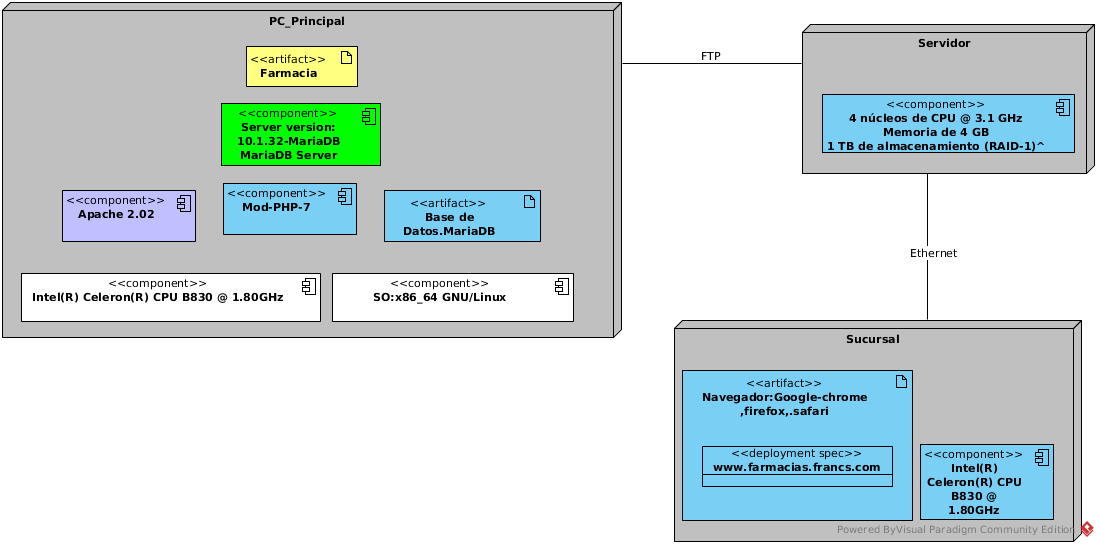
\includegraphics[width=.9\textwidth]{images/arquitectura}}
		\caption{Arquitectura del sistema.}
		\label{fig:arquitectura}
	\end{center}
\end{figure}

En la figura~\ref{fig:arquitectura} se describe la estructura del sistema, en ella se detalla los servicios de base de datos que se necesitan, las conexiones al servidor apache, así como las especificaciones que necesita el CPU de la sucursal en la que se monta el sistema de la farmacia.



